\documentclass[a4paper,twoside,12pt]{article}
\usepackage[T1]{fontenc}
\usepackage[utf8]{inputenc}
\usepackage[english]{babel}
\usepackage{enumerate}
\usepackage[shortlabels]{enumitem}
\usepackage{fullpage}
\usepackage{setspace}
\usepackage{graphicx}
\usepackage{import}
\usepackage{amsmath}
\usepackage{mathabx}
\usepackage{icomma}
\usepackage{booktabs}
\usepackage{ftcap}
\usepackage{lipsum}
\usepackage{url}
\usepackage[binary-units]{siunitx}
\usepackage{epstopdf}
\usepackage{hyperref}
\usepackage{subcaption}

\begin{document}
\onehalfspacing%
\thispagestyle{empty}
\begin{flushleft}
 \underline{Sakari} Matias Kapanen\hfill
 \texttt{sakari.m.kapanen@student.jyu.fi}
\end{flushleft}
\vfill
\begin{center}
\textsc{\LARGE FYSS430 A computer tomographic study of the infill ratio of a 3D printed object}
\end{center}
\vfill
Measurement date: January 25, 2017\\
Supervisor: Arttu Miettinen\\
\vfill
\begin{abstract}
 \noindent
    A three-dimensionally printed cube was scanned with a X-ray tomographic scanner in order to analyze the ratio of the infill material. Bruker SkyScan 1172 scanner was used. An analyzation code was devised to calculate the ratio through binary image processing. The resulting ratio was found to be 26-28 \% while the designed ratio was 20 \%. The disagreement was attributed to inaccuracy of the slicer software, miscalibration of the printer and edge effects.
\end{abstract}
\clearpage%

\setlength{\parindent}{0pt}
\setlength{\parskip}{12pt}

\setcounter{page}{1}

\section{Introduction}
Three-dimensional printing is an additive manufacturing method where plastic is extruded layer by layer to produce a three-dimensional object. A solid 3D CAD model is prepared for printing by a ``slicer'' software which generates the tool paths for the nozzle.

It does not often make sense to fill the whole solid model with plastic. Therefore a sparse ``infill'' pattern is generated instead as shown in image~\ref{fig:honeycomb}.

The volumetric ratio of the infill material inside the cube was chosen as the research subject of this computer tomography project work. Tomographic imaging makes it possible to acquire a volume image of the 3D printed cube which can be then analyzed by traditional image analysis methods.

\begin{figure}
    \centering
    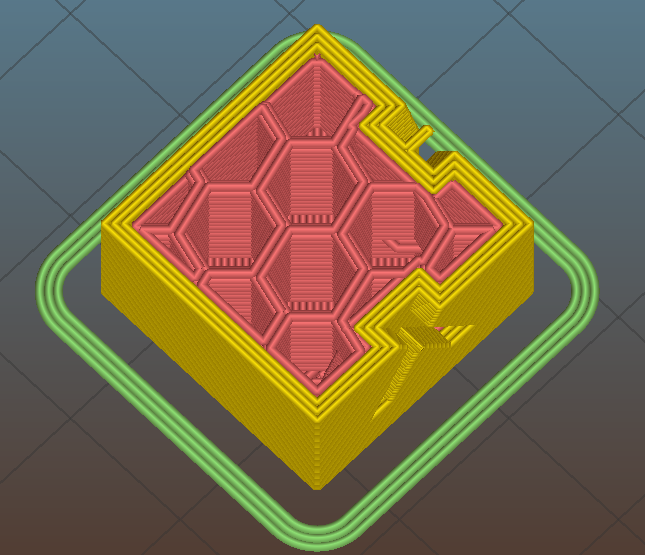
\includegraphics[width=0.8\textwidth]{images/cube_slic3r.png}
    \caption{A section of a three-dimensional cube model~\cite{testcube} sliced by Slic3r~\cite{slic3r}. A honeycomb infill pattern of 20 \% ratio has been generated inside.}
    \label{fig:honeycomb}
\end{figure}

\section{Theoretical background}
In this section, the theoretical foundations of computer tomographic imaging and image reconstruction are lightly covered. There is also a brief introduction to the image processing methods used.

In typical X-ray tomography scenarios, an X-ray beam is cast on the object to be imaged. On the other side there is a detector array. The object is mounted on a rotation stage. This allows taking X-ray projections of the object from different directions. From the two-dimensional projections, a volume image can be reconstructed.

\subsection{Beer-Lambert law}
The X-ray beams entering the target object are attenuated in the material. The attenuation can be attributed to various scattering phenomena taking place in the medium, most importantly photoelectric effect and Compton scattering~\cite{lectures}. The probability of these scatterings correlates to the density of the target material.

Consider a beam propagating in one dimension. In a simple linear model, the rate of the scatterings is proportional to the attenuation coefficient $\mu(x)$ and the beam intensity $I(x)$. On the other hand, the scatterings decrease the intensity. Therefore the change of intensity with respect to traveled distance can be written as
\begin{equation}
    \label{eq:bl_ode}
    \frac{\mathrm{d}I(x)}{\mathrm{d}x} = -\mu (x) I (x).
\end{equation}
This differential equation has a familiar solution of the form
\begin{equation}
    \label{eq:bl}
    I(x) = I_0 e ^ { -\int\limits_0^x \mu(x)\,\mathrm{d}x },
\end{equation}
where $I_0$ is the initial beam intensity. In the special case of a uniform medium, this becomes
\begin{equation}
    \label{eq:bl_linear}
    I(x) = I_0 e ^ { -\mu x }.
\end{equation}
Therefore it is seen that the beam exponentially decays in the medium. The thickness and the density of the medium therefore both contribute to the attenuation.

\subsection{Filtered backprojection}
Given a sufficient number of $Z$-projections, one can construct an image of the original volume. A simple method is to algebraically solve for the original voxel values using the projection data. However, this is inconvenient for any practical image sizes because the resulting equation group is large.

A more widely used, practical method is filtered backprojection. It is an integral transform based approach which is described in detail in~\cite{radon}. The basic idea is as follows:
\begin{enumerate}
    \item Each $Z$-slice is processed individually. The \emph{rows} of the projection images are considered as the projections of the respective slices, situated in the $XY$ plane.

    \item The series of projections of a single slice at different rotation angles are considered as the Radon transform of the slice.

    \item The Radon transform data is filtered in the Fourier domain by a ``ramp filter'' function $h(\omega) = |\omega|$ where $\omega$ is the frequency. This step has a high pass filtering effect and arises from the mathematics of the Radon transform.

    \item The filtered data is transformed with the inverse Radon transform. The result of the inverse transform is an image of the corresponding $Z$-slice.

    \item The procedure 2-4 is repeated for all slices, resulting in a volume image.
\end{enumerate}

Often, after the reconstruction process, the voxel values of the result are inverted such that larger values (brighter regions) correspond to volumes of greater density.

\subsection{Binary images and thresholding}
\label{sec:thresholding}
The volume image recovered by the reconstruction process is a greyscale image. To analyze different sections of the image, some kind of \emph{segmentation} has to be performed. One of the simplest cases of segmentation is the extraction of a light foreground from a dark background. In a simple case, the result of such an operation is a binary image where the foreground pixels are marked white and background pixels are marked black.

A binary mask like that can be achieved by thresholding: given a threshold value $t$, the thresholded image is given by
\begin{equation}
    \label{eq:threshold}
    g_t(\mathbf{x}) = \begin{cases}
        0 & \text{where } f(\mathbf{x}) \geq t \\
        1 & \text{where } f(\mathbf{x}) < t,
    \end{cases}
\end{equation}
where $f(\mathbf{x})$ is the original image. The thresholded image $g_t(\mathbf{x})$ has only values 0 and 1 and is thus called a \emph{binary} image.

The problem now boils down to finding the optimal threshold value which actually separates the foreground from the background. There are several automatic methods for obtaining such a threshold. One of them is the Otsu method~\cite{otsu}. In this method, the threshold is found as a solution to the optimization problem
\[
    \sigma_\text{B}^2(t_\text{Otsu}) = \max\limits_t \sigma_\text{B}^2(t),
\]
where $\sigma_\text{B}^2(t)$ is the between-class variance of the background and foreground pixel (or voxel) values of the respective pixel classes separated by the threshold $t$. This method works well if there are clear foreground and background peaks in the image histogram.

\subsection{Edge detection}
Another commonly useful image processing operation is edge detection. The notion of an edge usually corresponds to a discontinuity or a rapid change in the image. Therefore partial derivatives of the image are a natural way of finding the edges.

However, derivatives are also sensitive to noise in the image. Some low pass filtering of the image is usually performed to reduce noise. A useful property of convolution allows combining the derivative and the convolution operations:
\begin{equation}
    \frac{\partial}{\partial x} (f(x, y) \ast \mathbf{G}_\sigma) =
    f(x, y) \ast \frac{\partial}{\partial x} \mathbf{G}_\sigma,
\end{equation}
where $\mathbf{G}_\sigma$ is the Gaussian kernel with the width parameter $\sigma$ and $\ast$ is convolution. Thus, combined edge detection and low pass filtering can be done by convolving the image with kernel approximating the partial derivatives of the Gaussian function.

One can derive edge detection kernels of arbitrary sizes and accuracies. The Sobel kernels are a widely used approximation:
\begin{equation}
    \mathbf{G}_x = \begin{bmatrix}
        -1 & 0 & 1 \\
        -2 & 0 & 2 \\
        -1 & 0 & 1
    \end{bmatrix},
    \mathbf{G}_y = \begin{bmatrix}
        -1 & -2 & -1 \\
        0 & 0 & 0 \\
        1 & 2 & 1
    \end{bmatrix},
\end{equation}
which, while not greatly accurate, are an acceptable option if the desired result is achieved.

Given the values of the $x$ and $y$ partial derivatives, the magnitude of the gradient can be calculated as
\[
    \mathbf{G} = \sqrt{\mathbf{G}_x^2 + \mathbf{G}_y^2}.
\]
High values of the gradient magnitude signify the image edges.

\subsection{Morphological operations}
Morphological operations are a set of mathematical operations on binary images. The basic operations are \emph{erosion}, \emph{dilation}, \emph{opening} and \emph{closing}. All these operations involve the usage of a \emph{structuring element} which is a $n$-by-$m$ binary mask which determines the neighborhood that is sampled for each pixel during the operation.

Erosion and dilation are complementary: erosion shrinks white regions in the source image, dilation expands them (or shrinks black regions).

Opening is the chained operation of an erosion followed by a dilation. This removes white regions smaller than a certain size. Closing is the complement, which removes black regions smaller than a certain size.

These operations are widely implemented in popular image processing libraries and useful in manipulating binary images. For a more thorough explanation of them, see e.g. the OpenCV documentation~\cite{cv1, cv2}.

\section{Experimental methods}
The 3D printed sample was scanned with a Bruker SkyScan 1172 scanner~\cite{skyscan} and reconstructed with Bruker's NRecon software. The images were analyzed on a laptop computer. The entire analysis code is available at~\cite{code}.

\subsection{SkyScan 1172 CT scanner settings}
The sample was glued on a plastic rod which was mounted on a sample holder fixed on the rotational stage. The optimal settings were determined by inspecting preview images in the scanner control software. The X-ray voltage and current were chosen to yield sufficient dynamic range in the projection image while not overexposing it. No filter was used in the beam path. The most relevant settings and parameters are listed in table~\ref{table:settings}.

\begin{table}
    \centering
    \caption{Parameters used in scanning}
    \label{table:settings}
    \begin{tabular}{lr}
        \toprule
        Parameter name & Value \\
        \midrule
        X-ray source voltage & \SI{100}{\kilo\volt} \\
        X-ray source current & \SI{70}{\micro\ampere} \\
        Image pixel size & \SI{17.01}{\micro\meter} \\
        Angular step size & \SI{0.13}{\degree} \\
        Frame averaging & on, 17 frames \\
        Random movement & on, 20 \\
        \bottomrule
    \end{tabular}
\end{table}

A flat field was captured before scanning and used to remove the constant noise component from the frames. Frame averaging of 20 frames was used to reduce random noise in the images. In addition, the random movements feature was switched on in order to reduce ring artifacts.

The scan was done in two passes, one of which covering the bottom part of the sample and the other covering the top part. The individual scans were automatically stitched together in the software.

TODO add an example projection image

\subsection{Reconstruction}
Reconstruction was done in NRecon. Before the actual reconstruction, the reconstruction volume was roughly cropped based on the projection images to remove excess blank space.

Beam hardening correction, smoothing and ring artifact correction settings were chosen manually by bracketing the respective settings values and evaluating their effect on the preview image. The settings are listed in table~\ref{table:nrecon_settings}
\begin{table}
    \centering
    \caption{Parameters used in the NRecon reconstruction software}
    \label{table:nrecon_settings}
    \begin{tabular}{lr}
        \toprule
        Parameter name & Value \\
        \midrule
        Beam hardening correction & \SI{66}{\percent} \\
        Smoothing & 2 \\
        Smoothing kernel & Asymmetric boxcar \\
        Ring artifact correction & 12 \\
        \bottomrule
    \end{tabular}
\end{table}

An example of a reconstructed slice is shown in figure~\ref{fig:slice}. A three-dimensional visualization of the volume image is shown in~\ref{fig:volume_viewer}.
\begin{figure}
    \centering
    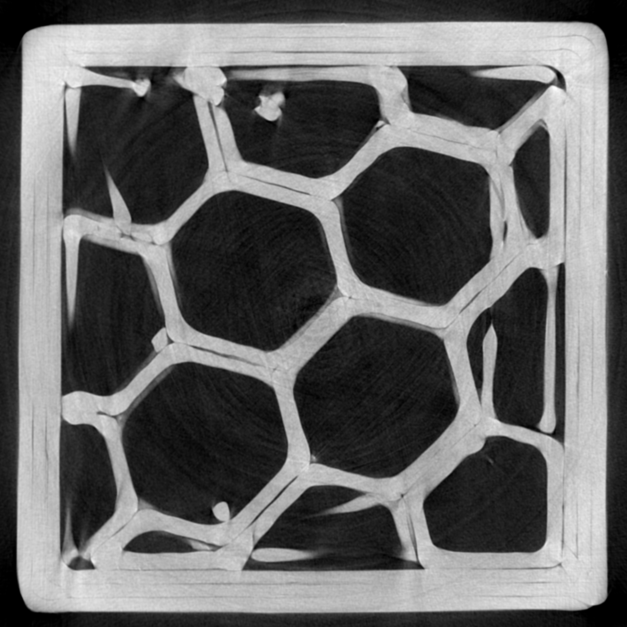
\includegraphics[width=0.8\textwidth]{images/slice_example.png}
    \caption{An example of a reconstructed slice of the volume image.}
    \label{fig:slice}
\end{figure}
\begin{figure}
    \centering
    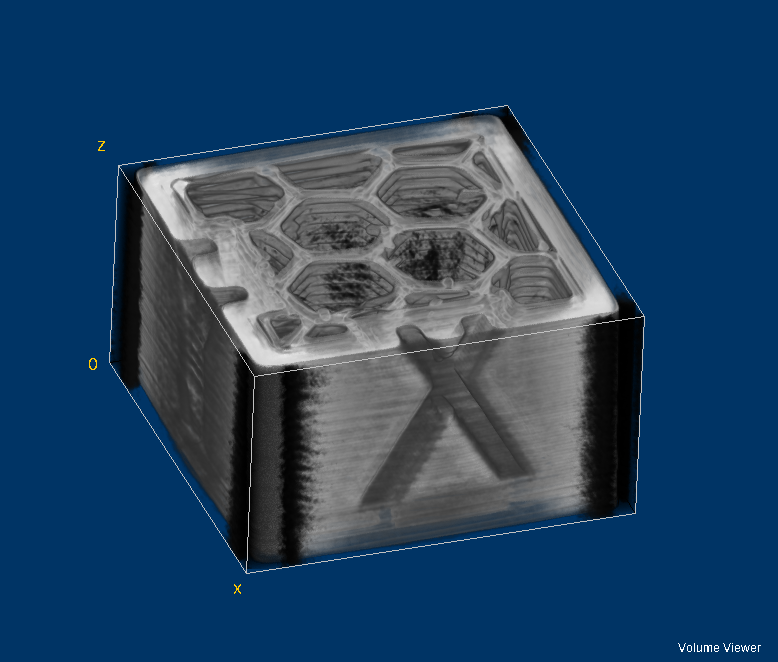
\includegraphics[width=0.8\textwidth]{images/volume_viewer.png}
    \caption{A 3D visualization reconstructed from the slices by Fiji Volume Viewer.}
    \label{fig:volume_viewer}
\end{figure}

\subsection{Image analysis software}
The tools of choice for performing the image analysis was \textsc{Python}~\cite{python} equipped with the libraries \textsc{scikit-image}~\cite{skimage} and \textsc{SciPy}~\cite{scipy}. These libraries provide a powerful software suite for analyzing N-dimensional images, including 3D image stacks resulting from CT scanning.

The image analysis was performed on a laptop computer with $\SI{4}{\giga\byte}$ of RAM. This initially posed some problems: the whole image stack was over $\SI{6}{\giga\byte}$. Therefore the full image could not be loaded in RAM, which made the image analysis practically impossible.

The problem was solved by discarding some information, for which the Fiji software suite~\cite{fiji} was used on a computer with sufficient RAM. An obvious first step was was to crop the image tighter than what was initially done -- there still was some blank space left in the volume image. The solid top and bottom of the cube were also excluded from the data already in this phase.

Second, the image was downscaled by a factor of 2 on each of the $XYZ$ axes. Finally, it was anticipated that the full 16 bits of bit depth would not be required. Thus, the bit depth was changed to 8 bits per pixel. The operations resulted to a sub-\SI{200}{\mega\byte} size of the full stack, which was far better workable on a laptop with low RAM.

\subsection{Segmentation}
To analyze the infill density, it was essential to be able to isolate the volume actually filled with the infill pattern.

In the 3D printed object, there is a vertical shell consisting of three extrudates. Therefore, the width of the outer shell remains relatively constant within and between slices. Hence, the following approach to processing the image was taken:
\begin{enumerate}
    \item Process the volume image slice-by-slice. This is a natural approach considering that the 3D printed object's features also appear on a slice-by-slice basis.
    \item Find the outer perimeter of the object using an edge detection method.
    \item If a consistent, continuous perimeter is found, mark it with white pixels.
    \item Fill the interior of the perimeter by white pixels using a flood fill operation, creating a binary image.
    \item \label{step:erosion} Offset the edge of the filled area inwards by a constant offset to reduce it so that it only covers to area filled with an infill pattern. This step can be realized using a morphological erosion operation.
\end{enumerate}
Upon completion, one has acquired a binary mask covering the areas with infill pattern.

In the edge detection step, a Sobel filter on the original greyscale image was initially used to find the magnitude of the image gradient. The greyscale image produced by Sobel was thresholded in order to mark the edge pixels as white.

However, the choice of a suitable threshold proved to be difficult. Sometimes the resulting edge would not be continuous, causing the flood fill operation to fail. On some other slices with the same threshold, reconstruction artifacts were taken as a part of the outer edge. Examples of both cases are presented in figure~\ref{fig:failed_sobel}.
\begin{figure}
    \centering
    \begin{subfigure}{0.5\textwidth}
        \centering
        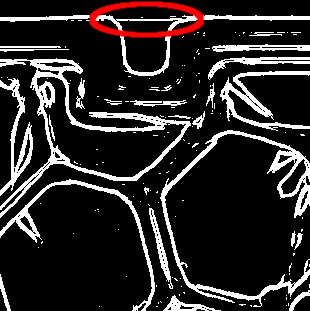
\includegraphics[width=0.8\linewidth]{images/sobel_binary_208.png}
    \end{subfigure}%
    \begin{subfigure}{0.5\textwidth}
        \centering
        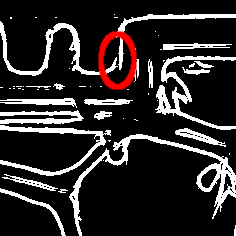
\includegraphics[width=0.8\linewidth]{images/sobel_binary_290.png}
    \end{subfigure}
    \caption{Two problematic cases of Sobel edge detection. On the left, a reconstruction artifact is treated as part of the outer perimeter. On the right, there is a discontinuity in the perimeter.}
    \label{fig:failed_sobel}
\end{figure}
A possible cure for the misidentified edges would be to increase the edge threshold value to exclude these. On the other hand, the small discontinuities could be fixed by a morphological closing operation.

Luckily, an even simpler method was found to perform very well in this case. In the images, there is a very consistent separation between the dark background and a foreground with close to uniform density. On such images, one can perform decent segmentation between background and foreground by generating a binary image. In particular, Otsu's automatic thresholding method performs very well on such occasions.

This was the case in this application. The Otsu method was used globally on the image stack in one pass and the volume image was thresholded. Inspecting the slices, the separation between background and foreground was clear and consistent across slices. An example is presented in figure~\ref{fig:otsu}.
\begin{figure}
    \centering
    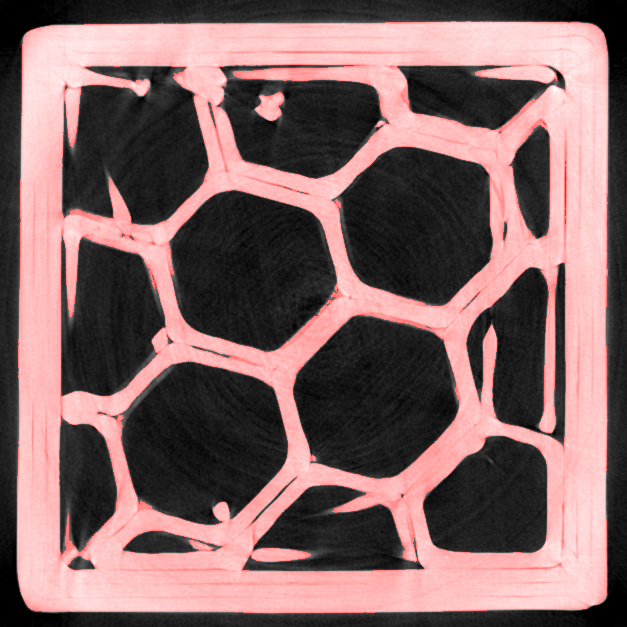
\includegraphics[width=0.8\textwidth]{images/binary_initial_24.png}
    \caption{An illustration of a binary mask generated using Otsu's method and thresholding. The foreground pixels (where the binary mask has value 1) are masked with red.}
    \label{fig:otsu}
\end{figure}
From there on, the flood fill operation produces the desired result where a pixel is marked white if and only if it is inside the outer perimeter.

The resulting mask was then shrinked as described in step~\ref{step:erosion}. A 5-by-5 square structuring element was found to give good results when the erosion operation was iterated several times. The more iterations are done, the more the mask is shrinked. An example is shown in figure~\ref{fig:eroded}.
\begin{figure}
    \centering
    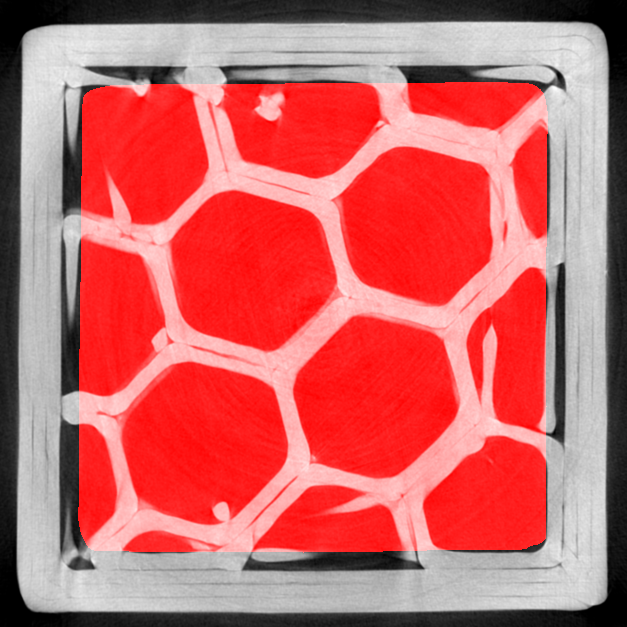
\includegraphics[width=0.8\textwidth]{images/eroded_24.png}
    \caption{An illustration of one slice of the final mask used to isolate the infilled region.}
    \label{fig:eroded}
\end{figure}

\subsection{Calculating the infill ratio}
Now that the region of interest has been found, the calculation of the actual infill ratio is left. To perform this calculation, a separation between background and foreground pixels is required. The Otsu thresholded binary image previously generated should be sufficient for this purpose.

A rigorous way of doing this calculation would be clipping ``sure'' background pixels to zero. Then the pixel values of the other pixels should be normalized according to the ``full density'' pixel value. Then the infill ratio would be achieved as
\[
    \text{infill ratio} = \frac{1}{N} \sum\limits_{\mathbf{x} \in \text{ROI}} f(\mathbf{x}),
\]
where $N$ is the number of voxels in the region where the infill density is evaluated (the set ROI) and $f(\mathbf{x})$ is the clipped and normalized image.

The advantage of this method is that if done right, it should take edge effects in account (where a voxel is only partially filled with material). However, this method requires some heuristics to find out the full density value. One choice would be to take the average of the pixel values on the perimeter (or some portion of it). Due to the normalization, the method is somewhat sensitive to the choice of this value.

A simpler method is to use the segmentation generated by Otsu thresholding. Then, an approximation of the infill ratio is
\begin{equation}
    \label{eq:infill_ratio}
    \text{infill ratio} = \frac{1}{N} \sum\limits_{\mathbf{x} \in \text{ROI}} g(\mathbf{x}),
\end{equation}
where $g(\mathbf{x})$ is the thresholded image and $N$ the number of voxels in the ROI. In this method, the Otsu method is implicitly responsible of the choice of normalization. As discussed in section~\ref{sec:thresholding}, the threshold chosen by the Otsu method is optimal in a statistical sense. Therefore, it should not be an entirely poor choice as an approximation.

\subsection{Pruning the slices}
In initial tests, it became evident that there were some problematic slices. In particular, there was a range of slices where some of the infill pattern was solid in order to support the above structures. An example is seen in figure~\ref{fig:solid_infill}. Since only the sparsely infilled regions are desired to be measured, that range of slices was excluded from the calculation. Luckily the range covered only 56 of the total of 353 slices.
\begin{figure}
    \centering
    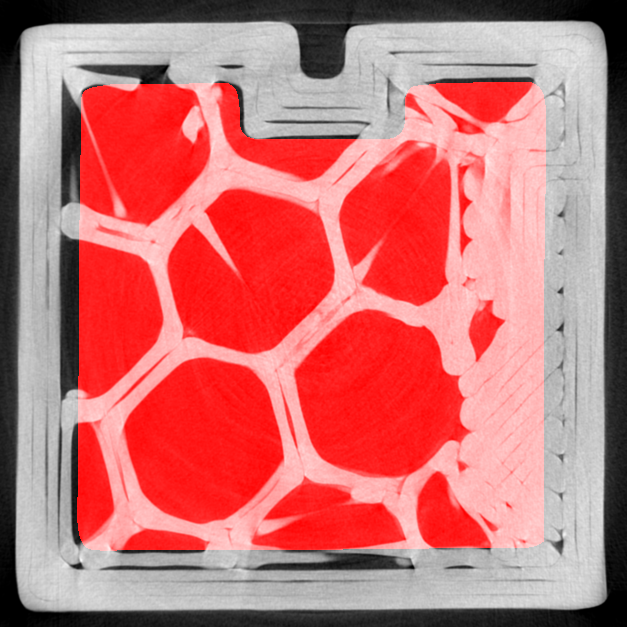
\includegraphics[width=0.8\textwidth]{images/eroded_71.png}
    \caption{An example of a slice that is partially filled with solid infill. The infill region mask is also shown.}
    \label{fig:solid_infill}
\end{figure}

\section{Results}
The infill ratio was evaluated using equation~\eqref{eq:infill_ratio} with several different choices of the ROI. The extent of the ROI was determined by the iteration count of erosions in the final step of forming the mask. The difference between iteration counts 30 and 50 is shown in figure~\ref{fig:erosion_count}.
\begin{figure}
    \centering
    \begin{subfigure}{0.5\textwidth}
        \centering
        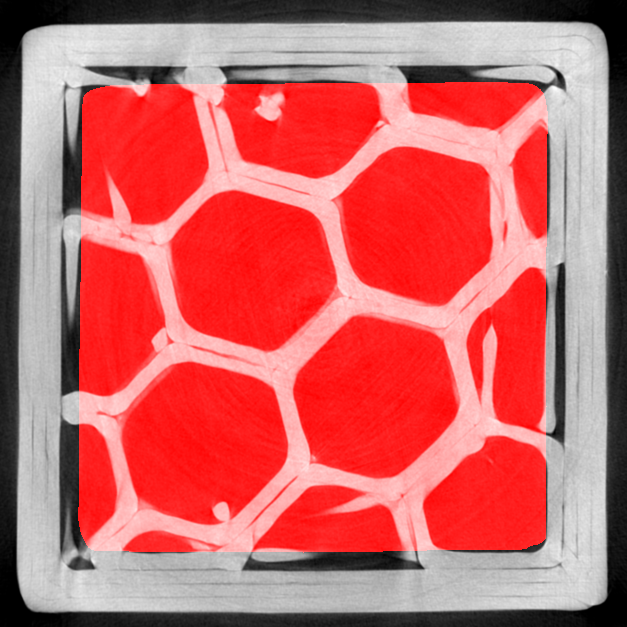
\includegraphics[width=0.8\linewidth]{images/eroded_24.png}
    \end{subfigure}%
    \begin{subfigure}{0.5\textwidth}
        \centering
        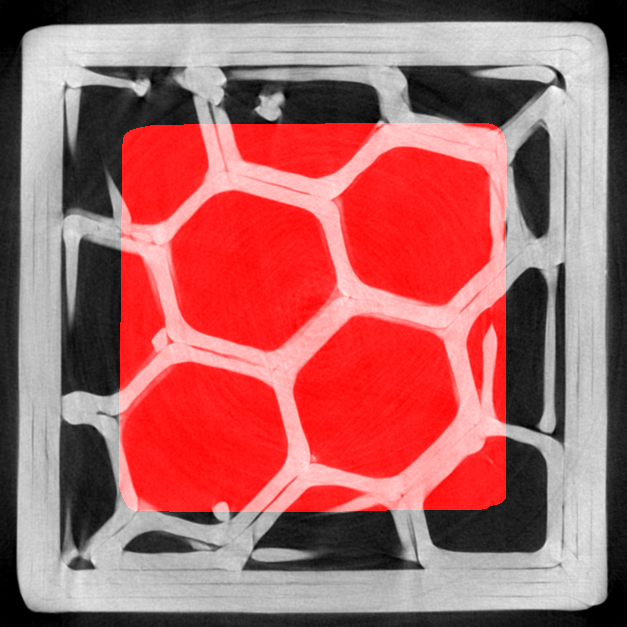
\includegraphics[width=0.8\linewidth]{images/eroded_24_50.png}
    \end{subfigure}
    \caption{On the left image, the erosion operation has been applied 30 times and on the right 50 times.}
    \label{fig:erosion_count}
\end{figure}
In table~\ref{table:results}, the resulting infill ratios are listed. The results are surprisingly coherent despite the different choices of the ROI. A reasonable estimate would be to say that the infill ratio is the range 26-28 \%.
\begin{table}
    \centering
    \caption{Calculated values of infill ratio using different numbers of erosion iterations.}
    \label{table:results}
    \begin{tabular}{lr}
        \toprule
        Erosion count & Infill ratio (\%) \\
        \midrule
        30 & 27.54 \\
        40 & 27.99 \\
        50 & 25.88 \\
        \bottomrule
    \end{tabular}
\end{table}

\section{Conclusions}
The infill ratio of 26-28 \% found above is in slight disagreement with the 20 \% ratio that was chosen in the slicer software. There are several equally potential contributors to the difference:
\begin{itemize}
    \item Inaccuracy of the slicer software. The user's choice of the infill ratio might be only approximate, and the actual density of the generated infill might depend on the shape and size of the volume to be filled.
    \item Miscalibration of the three-dimensional printer, causing too much material to be extruded.
    \item Edge effects: it would be better to sample a larger region of the infill pattern. This way one would get a more ``uniform'' look at the infill.
\end{itemize}
Additionally, equation~\eqref{eq:infill_ratio} is approximative. However, it is not believed to be a major source of deviation.

Setting the minor disagreement aside, this experiment proved that \textsc{Python} equipped with \textsc{scikit-image} and \textsc{SciPy} form a nice software suite for analyzing computer tomographic images.

It was also seen that through clever use of thresholding and morphological operations, one can create simple but effective image processing pipelines which achieve the desired result.

\clearpage

\begin{thebibliography}{9}
    \bibitem{testcube} XYZ 20mm Calibration Cube. User \emph{iDig3Dprinting}. \url{http://www.thingiverse.com/thing:1278865}. Referenced March 7, 2017.
    \bibitem{slic3r} Slic3r, G-code generator for 3D printers. \url{http://slic3r.org/}. Referenced March 7, 2017.
    \bibitem{lectures} FYSS430 X-ray tomography and image analysis, lecture notes. \emph{Arttu Miettinen}. University of Jyväskylä, 2017.
    \bibitem{radon} Applied Fourier Analysis and Elements of Modern Signal Processing, lecture notes. \emph{Emmanuel Candes}. Stanford University, 2016. \url{http://statweb.stanford.edu/~candes/math262/Lectures/Lecture09.pdf}. Referenced March 7, 2017.
    \bibitem{otsu} A Threshold Selection Method from Gray-Level Histograms. \emph{Nobuyuki Otsu}. IEEE Transactions on systems, man and cybernetics, vol. SMC-9, no. 1. January 1979.
    \bibitem{cv1} Eroding and Dilation. OpenCV 2.4.13 documentation. \url{http://docs.opencv.org/2.4/doc/tutorials/imgproc/erosion_dilatation/erosion_dilatation.html?highlight=morphology}. Referenced March 7, 2017.
    \bibitem{cv2} More Morphology Transformations. OpenCV 2.4.13 documentation. \url{http://docs.opencv.org/2.4/doc/tutorials/imgproc/opening_closing_hats/opening_closing_hats.html?highlight=morphology}. Referenced March 7, 2017.
    \bibitem{skyscan} SkyScan1172 | Bruker microCT. \url{http://bruker-microct.com/products/1172.htm}. Referenced March 8, 2017.
    \bibitem{python} Python. \url{https://www.python.org/}. Referenced March 8, 2017.
    \bibitem{skimage} scikit-image. \url{http://scikit-image.org/}. Referenced March 8, 2017.
    \bibitem{scipy} SciPy. \url{http://scipy.org/}. Referenced March 8, 2017.
    \bibitem{fiji} Fiji is just ImageJ. \url{http://fiji.sc/}. Referenced March 8, 2017.
    \bibitem{code} Analysis source code. \url{https://github.com/flannelhead/xray-tomography-project/blob/master/analysis/analyze.py}. Referenced March 8, 2017.
\end{thebibliography}
\end{document}

